\section{Results of the Runtime Verified AV System}

This research provides a solution for two aspects of \acf{AV} systems: predicting accurately with perturbations to the system's inputs and safely dealing with misclassifications by the system.
The issue of input perturbations was addressed using a \acf{MNN} of different convolutional \acfp{SNN}, each \ac{SNN} working in tandem to predict more accurately.
Misclassification by the system's controller was addressed by implementing sensor fusion between cameras and \ac{LiDAR}.
This was done using a run-time enforcer that enforced a safety automaton.

\todo{fix results with new graphs}

To test the \ac{MNN}'s ability to deal with perturbations, the input images (taken from the \ac{VOC} 2012 and \ac{GTSRB} datasets) were perturbed by randomly replacing approximately 7\% of the image pixels with randomly coloured pixels.
Table~\ref{tbl:sign-res} shows that without perturbations, the accuracy of the \ac{MNN} was increased from 87.07\% to 93.7\% when using an enforced policy.
Table~\ref{tbl:sign-respert} shows that the accuracy of the \ac{MNN} hugely decreases when perturbations are present, from 87.07\% to 41.6\%.
However, with sensor fusion and a relative safety policy, the accuracy is increased to 90.48\%.

\begin{table}[h]
	\centering
	\resizebox{\textwidth}{!}{%
		\begin{tabular}{|p{0.17\linewidth}||p{0.17\linewidth}|p{0.17\linewidth}|p{0.17\linewidth}|p{0.17\linewidth}|}
			\hline
			Epochs trained & No. of misclassifications (\%) & Caught misclassifications (\%) & False negatives (\%) & Uncaught misclassifications (\%) \\ \hline
			\multicolumn{5}{|l|}{Original Inputs} \\ \hline
			0 & 95.16 & 95.16 & 4.84 & 4.84 \\ 
			10 & 95.16 & 95.16 & 4.84 & 4.84 \\
			100 & 82.67 & 61.09 & 1.83 & 23.41 \\
			1000 & 29.36 & 21.39 & 2.92 & 10.89 \\
			10000 & 12.38 & 8.55 & 2.11 & 5.93 \\ 
			100000 & 11.98 & 7.79 & 2.13 & 6.33 \\
			6000 (best) & 10.59 & 7.32 & 2.04 & 5.31 \\ \hline
			\multicolumn{5}{|l|}{Perturbed Inputs} \\ \hline
			0 & 95.16 & 95.16 & 4.84 & 4.84 \\
			10 & 95.16 & 95.16 & 4.84 & 4.84 \\ 
			100 & 93.63 & 71.89 & 0.56 & 22.29 \\
			1000 & 76.69 & 63.71 & 1.25 & 14.23 \\
			10000 & 57.89 & 45.89 & 2.27 & 14.28 \\ 
			100000 & 58.03 & 45.72 & 2.39 & 14.69 \\
			7000 (best) & 60.42 & 49.13 & 2.20 & 13.49 \\ \hline
		\end{tabular}%
	}
	\caption{Table showing the results of the \ac{AV} prediction \ac{SNN}}
	\label{tbl:sign-resultsfull}
\end{table}


\begin{figure}[t]
	\centering
	\scalebox{1}{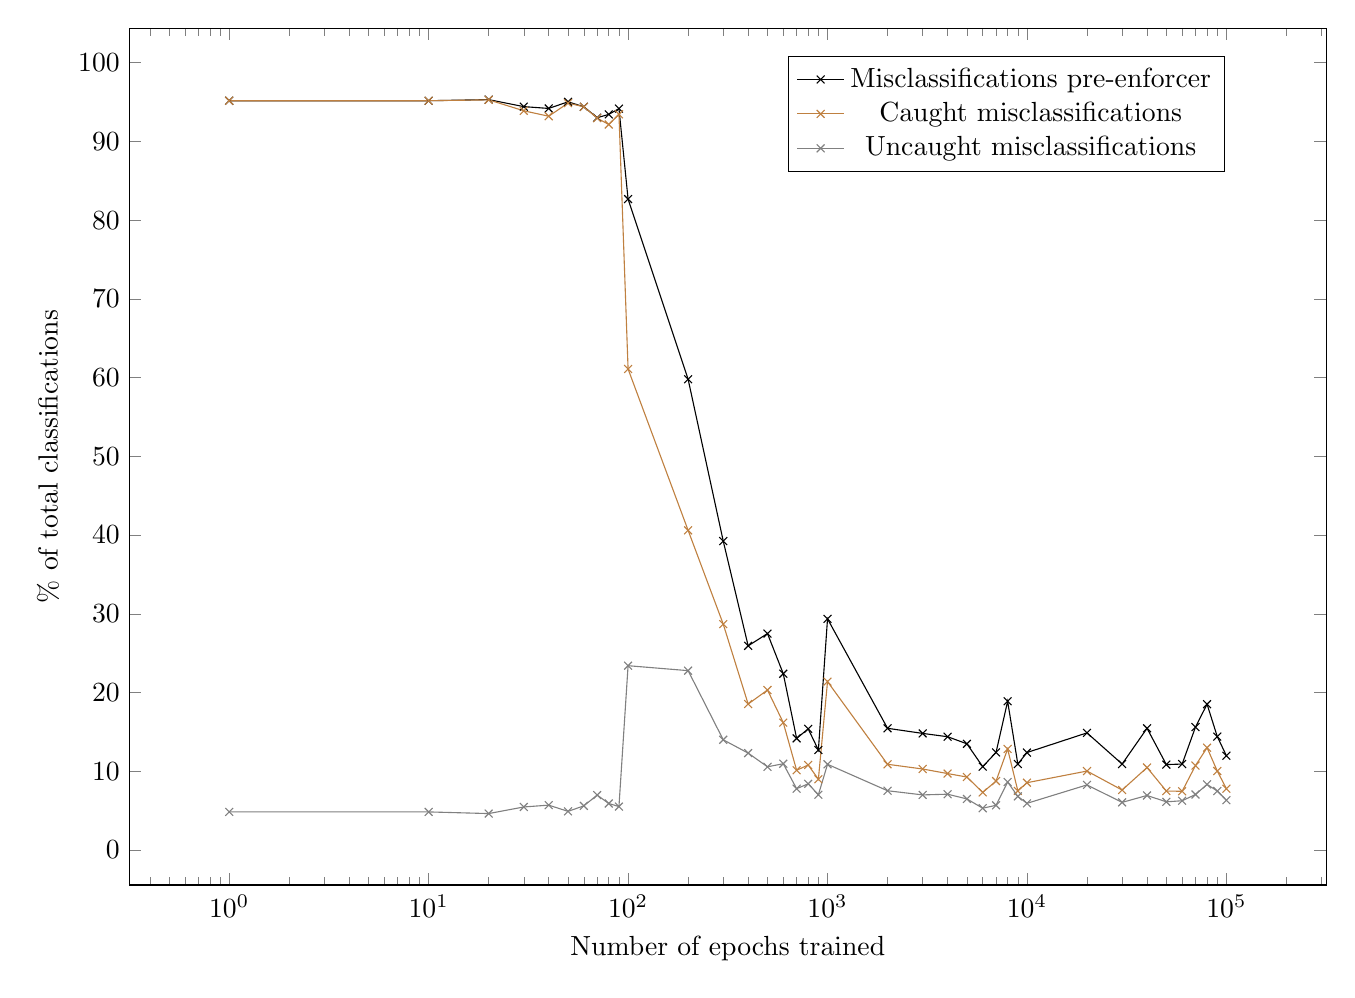
\begin{tikzpicture}
\begin{semilogxaxis}[
xlabel={Number of epochs trained},
ylabel={\% of total classifications},
x=1.1cm,
y=1.0mm, 
legend style={at={(0.55,0.9)},anchor=west}]

\addplot[color=black,mark=x] coordinates {
	(1, 95.159996)
	(10, 95.159996)
	(20, 95.300003)
	(30, 94.410004)
	(40, 94.180000)
	(50, 95.019997)
	(60, 94.389999)
	(70, 93.000000)
	(80, 93.419998)
	(90, 94.159996)
	(100, 82.669998)
	(200, 59.790001)
	(300, 39.240002)
	(400, 25.930000)
	(500, 27.490000)
	(600, 22.389999)
	(700, 14.180000)
	(800, 15.390000)
	(900, 12.700000)
	(1000, 29.359999)
	(2000, 15.460000)
	(3000, 14.810000)
	(4000, 14.390000)
	(5000, 13.490000)
	(6000, 10.590000)
	(7000, 12.400000)
	(8000, 18.889999)
	(9000, 10.920000)
	(10000, 12.380000)
	(20000, 14.880000)
	(30000, 10.920000)
	(40000, 15.460000)
	(50000, 10.850000)
	(60000, 10.920000)
	(70000, 15.620001)
	(80000, 18.520000)
	(90000, 14.410000)
	(100000, 11.980000)
};

\addplot[color=brown,mark=x] coordinates {	
	(1, 95.159996)
	(10, 95.159996)
	(20, 95.269997)
	(30, 93.880005)
	(40, 93.189995)
	(50, 94.860001)
	(60, 94.389999)
	(70, 92.950005)
	(80, 92.139999)
	(90, 93.440002)
	(100, 61.090000)
	(200, 40.599998)
	(300, 28.690001)
	(400, 18.540001)
	(500, 20.320000)
	(600, 16.180000)
	(700, 10.130000)
	(800, 10.800000)
	(900, 8.990000)
	(1000, 21.389999)
	(2000, 10.890000)
	(3000, 10.290000)
	(4000, 9.710000)
	(5000, 9.270000)
	(6000, 7.320000)
	(7000, 8.760000)
	(8000, 12.840000)
	(9000, 7.510000)
	(10000, 8.550000)
	(20000, 10.030000)
	(30000, 7.620000)
	(40000, 10.480000)
	(50000, 7.490000)
	(60000, 7.460000)
	(70000, 10.730000)
	(80000, 13.000000)
	(90000, 10.030000)
	(100000, 7.790000)
};

\addplot[color=gray,mark=x] coordinates {
	(1, 4.840000)
	(10, 4.840000)
	(20, 4.630000)
	(30, 5.470000)
	(40, 5.700000)
	(50, 4.910000)
	(60, 5.610000)
	(70, 6.980000)
	(80, 5.910000)
	(90, 5.520000)
	(100, 23.410000)
	(200, 22.780001)
	(300, 14.000000)
	(400, 12.310000)
	(500, 10.570000)
	(600, 10.960000)
	(700, 7.790000)
	(800, 8.410000)
	(900, 7.020000)
	(1000, 10.890000)
	(2000, 7.530000)
	(3000, 7.000000)
	(4000, 7.090000)
	(5000, 6.490000)
	(6000, 5.310000)
	(7000, 5.680000)
	(8000, 8.640000)
	(9000, 6.810000)
	(10000, 5.930000)
	(20000, 8.270000)
	(30000, 6.050000)
	(40000, 6.930000)
	(50000, 6.120000)
	(60000, 6.260000)
	(70000, 7.050000)
	(80000, 8.340000)
	(90000, 7.490000)
	(100000, 6.330000)
};

\legend{Misclassifications pre-enforcer, Caught misclassifications, Uncaught misclassifications}
\end{semilogxaxis}%
\end{tikzpicture}%}
	\caption{Line graph showing the performance of the system trained over an increasing amount of epochs using unperturbed inputs \label{fig:sign-graph}}
\end{figure}

\begin{figure}[t]
	\centering
	\scalebox{1}{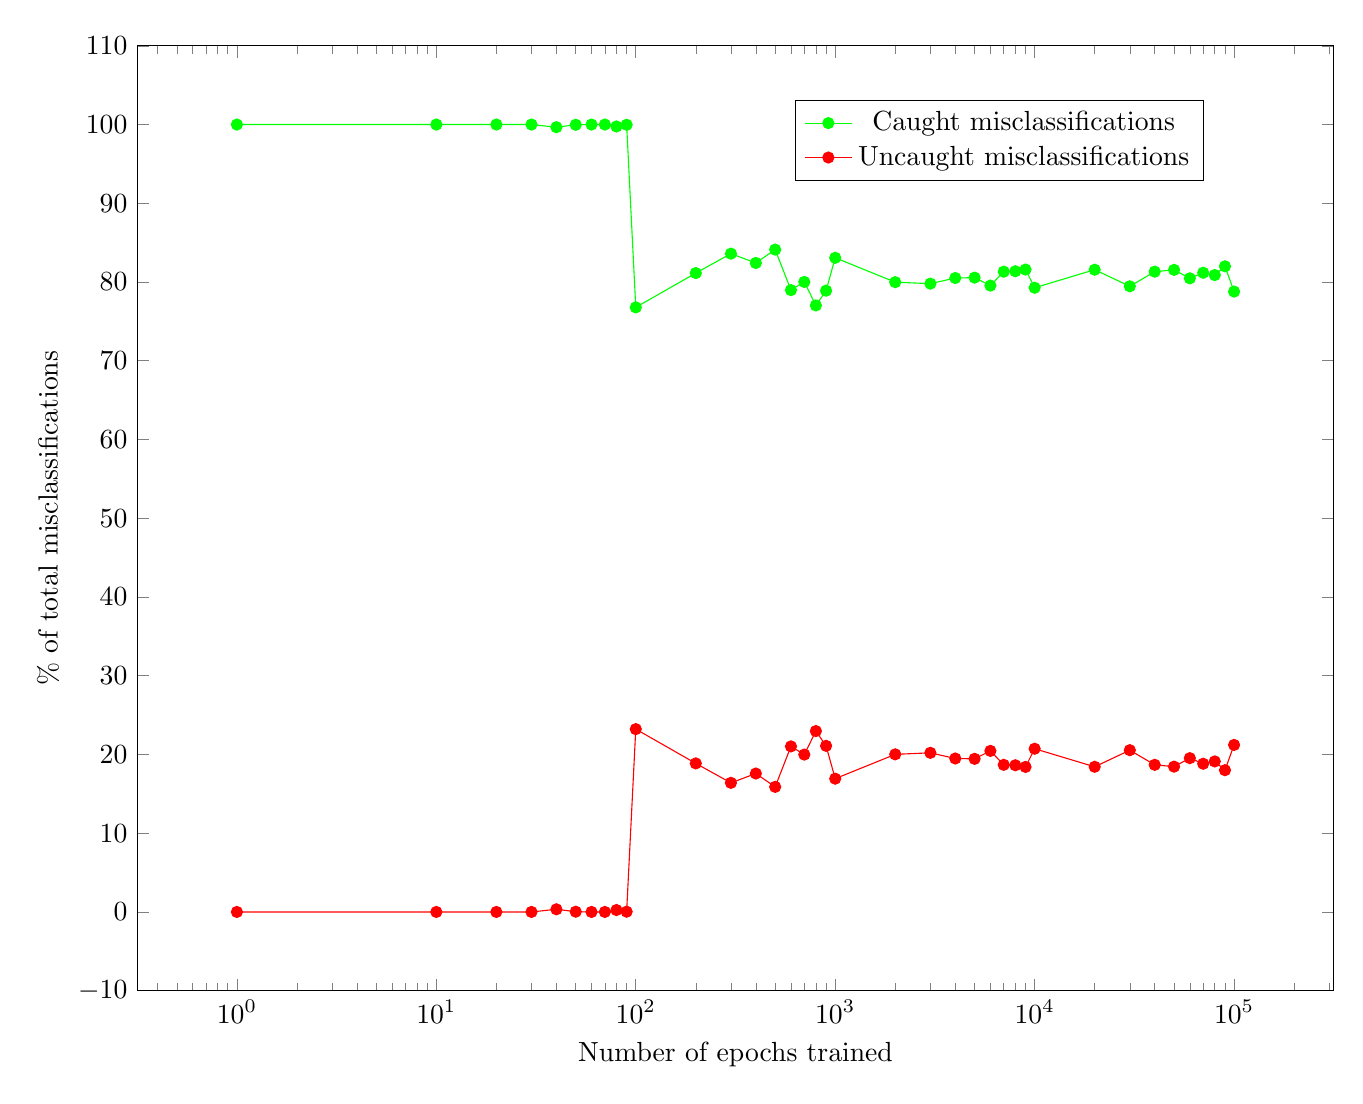
\begin{tikzpicture}
\begin{semilogxaxis}[
xlabel={Number of epochs trained},
ylabel={\% of total misclassifications},
x=1.1cm,
y=1.0mm, 
legend style={at={(0.55,0.9)},anchor=west}]

\addplot[color=green,mark=*] coordinates {	
	(1, 100.000000)
	(10, 100.000000)
	(20, 100.000000)
	(30, 100.000000)
	(40, 99.662552)
	(50, 99.968597)
	(60, 100.000000)
	(70, 100.000000)
	(80, 99.758133)
	(90, 99.968475)
	(100, 76.780945)
	(200, 81.134331)
	(300, 83.604851)
	(400, 82.419716)
	(500, 84.116234)
	(600, 78.973373)
	(700, 80.015221)
	(800, 77.028572)
	(900, 78.905663)
	(1000, 83.074722)
	(2000, 79.983315)
	(3000, 79.792389)
	(4000, 80.510559)
	(5000, 80.555107)
	(6000, 79.547066)
	(7000, 81.314125)
	(8000, 81.369659)
	(9000, 81.582603)
	(10000, 79.271027)
	(20000, 81.565376)
	(30000, 79.456421)
	(40000, 81.315414)
	(50000, 81.545204)
	(60000, 80.468216)
	(70000, 81.178162)
	(80000, 80.884285)
	(90000, 81.995102)
	(100000, 78.786835)
};

\addplot[color=red,mark=*] coordinates {
	(1, 0.000000)
	(10, 0.000000)
	(20, 0.000000)
	(30, 0.000000)
	(40, 0.337446)
	(50, 0.031402)
	(60, 0.000000)
	(70, 0.000000)
	(80, 0.241872)
	(90, 0.031525)
	(100, 23.219051)
	(200, 18.865665)
	(300, 16.395145)
	(400, 17.580284)
	(500, 15.883766)
	(600, 21.026627)
	(700, 19.984774)
	(800, 22.971428)
	(900, 21.094332)
	(1000, 16.925280)
	(2000, 20.016680)
	(3000, 20.207613)
	(4000, 19.489441)
	(5000, 19.444899)
	(6000, 20.452932)
	(7000, 18.685873)
	(8000, 18.630341)
	(9000, 18.417391)
	(10000, 20.728970)
	(20000, 18.434624)
	(30000, 20.543579)
	(40000, 18.684584)
	(50000, 18.454794)
	(60000, 19.531784)
	(70000, 18.821840)
	(80000, 19.115713)
	(90000, 18.004898)
	(100000, 21.213161)
};

\legend{Caught misclassifications, Uncaught misclassifications}
\end{semilogxaxis}%
\end{tikzpicture}%}
	\caption{Line graph showing the number of misclassifications made by the system with perturbed inputs \label{fig:sign-graphpert}}
\end{figure}

\begin{figure}[t]
	\centering
	\scalebox{1}{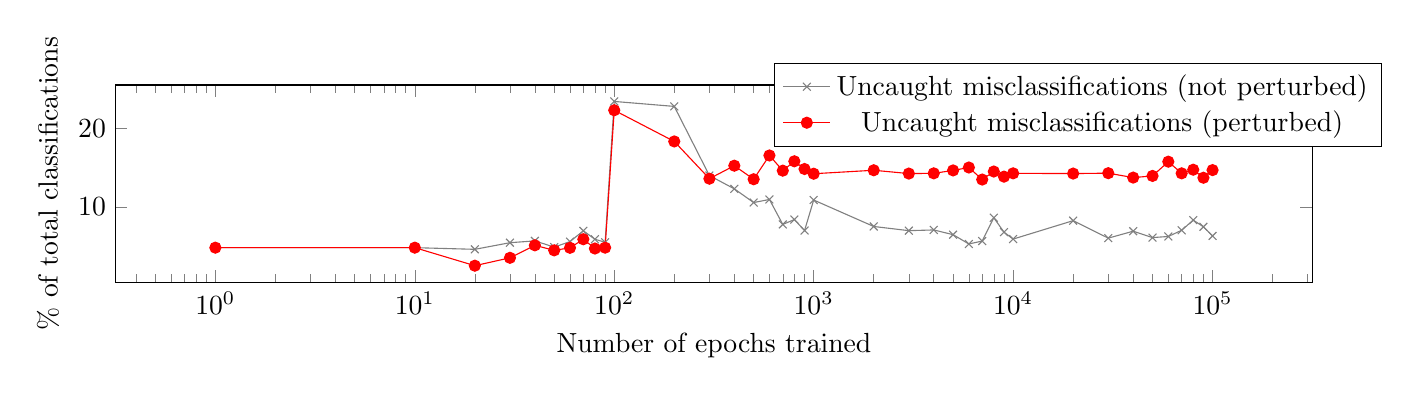
\begin{tikzpicture}
\begin{semilogxaxis}[
xlabel={Number of epochs trained},
ylabel={\% of total classifications},
x=1.1cm,
y=1.0mm, 
legend style={at={(0.55,0.9)},anchor=west}]

\addplot[color=gray,mark=x] coordinates {
	(1, 4.840000)
	(10, 4.840000)
	(20, 4.630000)
	(30, 5.470000)
	(40, 5.700000)
	(50, 4.910000)
	(60, 5.610000)
	(70, 6.980000)
	(80, 5.910000)
	(90, 5.520000)
	(100, 23.410000)
	(200, 22.780001)
	(300, 14.000000)
	(400, 12.310000)
	(500, 10.570000)
	(600, 10.960000)
	(700, 7.790000)
	(800, 8.410000)
	(900, 7.020000)
	(1000, 10.890000)
	(2000, 7.530000)
	(3000, 7.000000)
	(4000, 7.090000)
	(5000, 6.490000)
	(6000, 5.310000)
	(7000, 5.680000)
	(8000, 8.640000)
	(9000, 6.810000)
	(10000, 5.930000)
	(20000, 8.270000)
	(30000, 6.050000)
	(40000, 6.930000)
	(50000, 6.120000)
	(60000, 6.260000)
	(70000, 7.050000)
	(80000, 8.340000)
	(90000, 7.490000)
	(100000, 6.330000)
};

\addplot[color=red,mark=*] coordinates {
	(1, 4.840000)
	(10, 4.840000)
	(20, 2.550000)
	(30, 3.550000)
	(40, 5.140000)
	(50, 4.500000)
	(60, 4.820000)
	(70, 5.910000)
	(80, 4.730000)
	(90, 4.840000)
	(100, 22.290001)
	(200, 18.330000)
	(300, 13.600000)
	(400, 15.250000)
	(500, 13.530000)
	(600, 16.549999)
	(700, 14.620001)
	(800, 15.810000)
	(900, 14.830000)
	(1000, 14.230000)
	(2000, 14.670000)
	(3000, 14.250000)
	(4000, 14.280000)
	(5000, 14.650001)
	(6000, 15.020000)
	(7000, 13.490000)
	(8000, 14.510000)
	(9000, 13.860001)
	(10000, 14.280000)
	(20000, 14.250000)
	(30000, 14.300000)
	(40000, 13.740000)
	(50000, 13.950000)
	(60000, 15.760000)
	(70000, 14.280000)
	(80000, 14.740000)
	(90000, 13.720000)
	(100000, 14.690001)
};

\legend{Uncaught misclassifications (not perturbed), Uncaught misclassifications (perturbed)}
\end{semilogxaxis}%
\end{tikzpicture}%}
	\caption{Line graph showing the number of misclassifications made by the system with all inputs \label{fig:sign-graphboth}}
\end{figure}

%\todo{Add table showing how \ac{MNN} affects the prediction accuracy}

\subsection{An \ac{AV} System Using \acf{MNN2C}}
\ac{MNN2C}, introduced in Section~\ref{sec:mnn2c}, creates time-predictable, modular \acfp{MNN} for C from existing Keras (with Tensorflow) trained \acp{ANN}. 
This compiler makes implementing \acfp{SNN} in C easy and safe.
For the purposes of testing and demonstration, the complex \ac{MNN} used in this chapter, shown in Figure~\ref{fig:mnn}, was trained in Python, using Keras and the exact same images used to train the original system.
This \ac{MNN} was then described in the \ac{MNN2C} format, and modular C code was generated to initialise, run and incorporate the \ac{MNN}.
To show the efficacy of \ac{MNN2C}, the generated \ac{MNN} was implemented in an identical system to the original, and run with the same tests. 
It has already been shown that \ac{MNN2C} generates outputs identical to the Keras trained \acp{ANN} with a one hundred-thousandth tolerance, so the output of each individual \ac{ANN} is not being tested, rather that the system as a whole runs as the original does.
Additionally, the time-predictable \ac{MNN} was run through the Patmos \ac{WCET} tool in order to get the \ac{WCET} and \ac{WCRT} of the \ac{MNN}.

\subsubsection{Results of an \ac{MNN2C} Generated \ac{AV} System}
\begin{table}[h]
	\centering
	\resizebox{\textwidth}{!}{%
		\begin{tabular}{|p{0.17\linewidth}||p{0.17\linewidth}|p{0.17\linewidth}|p{0.17\linewidth}|p{0.17\linewidth}|}
			\hline
			Epochs trained & No. of misclassifications (\%) & Caught misclassifications (\%) & False negatives (\%) & Uncaught misclassifications (\%) \\ \hline
			\multicolumn{5}{|c|}{Original Inputs} \\ \hline
			100 & 25.01 & 24.22 & 17.50 & 18.29 \\ \hline
			\multicolumn{5}{|c|}{Perturbed Inputs} \\ \hline
			100 & 41.95 & 39.61 & 21.44 & 23.78 \\ \hline 
		\end{tabular}%
	}
	\caption{Table showing the results of the \ac{AV} prediction \ac{SNN}}
	\label{tbl:sign-resultsfullmnn2c}
\end{table}





















